\documentclass{llncs}
\usepackage{makeidx}
\setcounter{tocdepth}{2}
\title{Symbolic Music Similarity}
\author{Ali Bektas \and Paul Kröger}
\date{April 2020}


\usepackage{graphicx}
\graphicspath{{./img/}}

\usepackage{verbatim}
\usepackage{mathtools}


%Eine Ausarbeitung hat einen Titel, einen (oder mehrere) Verfasser, einen Betreuer, ein
%Erstellungsdatum und ist in einem Seminar in einem Jahr verfasst worden. Geben Sie das
%alles auf einer Titelseite an. 
\title{Symbolic Melodic Music Similarity}
\titlerunning{Symbolic Music Similarity}
	\author{Ali Bektas \and Paul Kröger \\ \textbf{Betreuer :} Prof. Dr. Ulf Leser \\ Similarity Search \\ WS19-20}
	%TODO : Man sollte hier noch das Datum einfügen.
	\date{\today}
  	\institute{ \vspace{5px} 
  	Humboldt Universität zu Berlin\\}
	



\begin{document}



    
    \let\oldaddcontentsline\addcontentsline
    \def\addcontentsline#1#2#3{}
    \mainmatter
    \maketitle
    \def\addcontentsline#1#2#3{\oldaddcontentsline{#1}{#2}{#3}}

	\tableofcontents
	
	\begin{abstract}
	With an increasing need to compare symbolic musical data in terms of their content 
	the question of similarity between musical objects becomes a challenge. While 
	there is not a single similarity function to answer all different needs , various approaches
	have been introduced to the field in recent decades. In our paper , we introduce the approaches
	which focus on symbolic melodic data , that is , a representation of the melody of a piece based on an alphabet
	of symbols and syntax. We discuss why this particular field had seen a trend to move towards geometrical approaches rather than those that are used by text-based similarity measures. As the leading algorithm in this field , we examine Melody-Shape algorithm and its success in MIREX competitions.
	\end{abstract}

	\section{Introduction}
		Similarity measures lie at the heart of Information Retrieval. This is also the case for melodic music similarity. For a subscriber of a music streaming application like Spotify , Last.fm etc. to recommend latest albums or a musicologist to find related documents in a database , similarity measures are crucial. In comparison to its counterpart Audio Music Similarity , Symbolic Music Similarity algorithms use symbols that represent the data , where in Audio Music Similarity one has pitch-time related values. Within Symbolic Music Similarity we find algorithms that deal with harmony and those that deal with melody. What differs harmony from melody is that by harmony we see chords , that is multiple notes played at a discrete time $t$ that together form a unity.  

		Representation of music dates back to as early as 2000 BC \cite{kil:civ}. Representing music over an alphabet consists in describing the pitch and the rhythm. Since we are mainly concerned with Western music , we can restrict ourselves to 12 tones of an octave , other cultures however may use more or less notes. In Middle Eastern countries ,for instance , we see that there are 9 tones between two notes of a whole tone interval.

		In further sections we will introduce some algorithms which implement basic text-similarity related operations to conclude similarity between melodies. That being said , we will also introduce  algorithms , that treat musical data different than text-similarity algorithms would treat  strings. The MelodyShape Algorithm of J. Urbano \cite{five_point_two}  and its variations give the best results in MIREX's (Music Information Retrieval Evaluation EXchange) annual competitions , between years 2010-2015
		%TODO
		Urbano's MelodyShape forms spline-sequence for the query melody and compares it with other spline-sequences to determine similarity between pieces. We will conclude from this , that the field evolved in recent years in such a way that the text-based approaches are less promising for the future of the field.

		Other than MelodyShape and its variations we will also present a graph-based approach \cite{two_point_four} , which incorporates routines to generalize the melody, that heavily depend on Music Theory , and a geometrical approach which use polygonal chains that are built by projecting the melody onto a plain of pitch and duration.

		In our paper we will follow the classification used by Velardo et al. \cite{two}. According to Velardo et al. a melodic music similarity algorithm belongs to either of the four classes (1) Music Theory , (2) Cognition , (3) Mathematics or (4) Hybrid. Hybrid algorithms are usually formed by taking a linear combination of different similarity measures. 

		Our main emphases are that the field suffers from the subjectivity of music similarity and that one single algorithms fails to answer all needs , which is especially the case when algorithms are tested only against a narrow range of data. In order to reduce these drawbacks we will show how MIREX , an EXchange group for Music Information Retrieval , took statistical approaches to form a Ground Truth for the data , that were collected from experts' evaluations. 
	
	\section{Algorithms}

		\subsection{A Graph Based Approach}

		Orio et al. \cite{two_point_four} introduce in their paper a series of operations to reduce melodies into a single large tree. Melodies are segmentated and then these segments are added into the tree as terminal nodes. The intermediate nodes represent generalization of the segments. 
		In a single step of generalization a segment is transformed into a simpler segment by deleting less important notes in the given segment. Which notes are less important is decided by three weight coefficents : \textit{(1)} its underlying harmonic function, \textit{(2)} its metric position  and \textit{(3)} the interval between the tone and the root of the underlying chord. 
		In order to determine these coefficients, harmonic analysis must be applied. Harmonic analysis is the process of making statements about in which way notes of a sequence are related to each other. These three coefficents must then be determined in such a way that it reflects the priorities of the human when considering two songs to be similar. 
		In their paper Orio et al. state that they chose to manually annotate the functions of notes in order to prevent any problems that could have otherwise arised during automated annotation , which could cause wrong simplification steps. We see this as a serious challange for the data , that only contain melody in comparison to data with harmonic elements, which could give better results of the underlying harmony. 

		The distance between two documents is expressed as the median of shortest distance between all segments. The similarity function $s(c_i , q)$ between a document $c_i$ from a collection of $N$ documents and a query document q is calculated as :
		
		\begin{equation}
			s(c_i , q)= 1 + \frac{d(c_i , q)}{\sum_{j=1}^{N} \frac{d(c_i,c_j)}{N-1}} 
		\end{equation}

		The similarity function is normalized and authors mention that 'the normalization factors can be computed off-line to speed up retrieval'. Authors also mention that the tree representation can offer novel ways to view a collection and see visually to what extent two songs were considered to be similar.


		\subsection{Urbano Melody-Shape}
        In 2010 J.Urbano et al. proposed a new method to calculate similarity between symbolic melodic pieces, comparing the shapes of melodies created by looking at notes as points on a pitch-time plane and interpolating a curve through those points \cite{five_point_five}.
           \begin{figure}[h!]
			\centering
        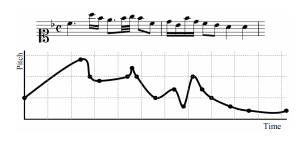
\includegraphics[width=200px,height=100px,keepaspectratio]{one_of_five_point_one}
			\caption{Notes represented as a curve on a pitch-time plane \cite{five_point_two}}
        \end{figure}
        Based on this method Urbano developed two algorithms for the MIREX Competition, Shape (in three variants: ShapeL, ShapeG and ShapeH) which only uses the pitch dimension and Time which uses both the pitch and the time dimension \cite{five_point_two}. Both algorithms seperate melodies into sequences of notes, and use Uniform B-Splines to get a spline sequence representation. Two spline sequences are then compared using sequence alignment. Based upon the results of the first Mirex competitions Urbano entered he also developed the ShapeTime system, which collects the n most relevant documents out of the data set, against which the query is run, using the ShapeH system and then ranks those documents using the time system. This was done because the ShapeH system performed better in rank unaware measures, whilst the time system performed better in rank aware measures in the competition. The ShapeTime system usually achieved the best overall results, as we will show later in the evaluation section.
        \subsubsection{ShapeH} 
        This system ignores the time dimension and only focuses on the shape of a melody. It uses spline-span sequences 3 notes long which results in a polynomial of degree 2 for each spline. They are then differentiated, resulting in polynomials of degree 1. 
        A dynamic programming table is then filled using a global alignment algorithm. The score of a cell (i,j) is computed by : \\
        $H(i,j) = max $
       $\begin{Bmatrix*}[c]
        H(i-1, j-1) + s(a_i, b_j) \\
        H(i-1,j) + s(a_i, -) \\
        H(i, j-1) + s(-,b_j)
        \end{Bmatrix*}$
		\\
		where H is the dynamic programming table, a and b the compared spline-span sequences. The highest score from the table is then used as the similarity score between the melodies. This hybrid alignment approach is used in favor of just the global alignment algorithm because Urbano argues that listeners put more emphasis on the beginning of a melody rather than the end when determining similarity. \\
		The operations are defined as follows : 
        \begin{itemize}
         \item Insertion : 
        $ s(-,n) = -(1-f(n)).$
        \item Deletion : 
         $s(n,-) = -(1 - f(n))$
        \item Match : 
        $s(n,n) = 1-f(n)$
        \end{itemize}
        
        Where f(n) denotes the frequency of a spline in the spline-span sequence. Urbano argues that the more often a spline occurs, the less important it is for the comparison. \\
        The substitution or mismatch score is calculated based on the shape of the spans where two melodies with a similar shape only get a small penalization. There are three possible scenarios : 
        \begin{itemize}
         \item If the derivative sign at the start and at the end of the splines are the same, they are considered to have a similar shape and there is only a small penalization.
         \item If the derivative sign only matches at the start or the end of the splines, they are considered to be less similar and there is a medium penalization.
         \item If the derivative sign at the start and the end of the spline does not match, they are considered to be not similar and there is a large penalization.
        \end{itemize}
        Due to looking at polynomials of degree 2 it is sufficient to only regard the start and end points of the splines, because they can only change their direction once within the span.
        It should be noted here that Urbano also submitted the ShapeG and ShapeL systems to Mirex competitions, which only differ from the ShapeH system in that they use a strictly global and a strictly local alignment approach, respectively, instead of the hybrid alignment approach. However the ShapeH system on average produced the best results in the Mirex competitions as we will show later.
  
		
		\subsubsection{Time}
        \begin{figure}[h!]
			\centering
		  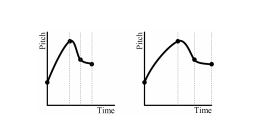
\includegraphics[width=200px,height=100px,keepaspectratio]{two_of_five_point_one}
			\caption{Normalization of spline \cite{five_point_two}}
        \end{figure}
        This system uses the time dimension as well and calculates the area between splines to determine similarity. It uses spline-span sequences 4 notes long which results in a polynomial of degree 3 for each spline. They are then differentiated, resulting in polynomials of degree 2. Each span duration is normalized to the same length. (Fig 2)
        It uses the same hybrid allignement approach as the ShapeH system. 
		The operations are defined as follows : 
        \begin{itemize}
         \item Insertion : 
        $ s(-,n) = -diff _p(n, \phi(n)) - \lambda k_t * diff_t(n, \phi(n)).$
        \item Deletion : 
         $s(n,-) = -diff_p(n, \phi(n)) - \lambda k_t * diff_t (n, \phi(n)).$
       \item substitution : 
       $s(n,m) = - diff_p (n,m) - \lambda k_t * diff_t (n,m) $
       \item Match : 
        $s(n,n) = 2\mu_p + 2\lambda k_t \mu_t = 2\mu_p (1+k_t).$
        \end{itemize}
        
        $diff_p$ and $diff_t$ are defined as the area of the compared first derivatives from the splines pitch and time function.$ \phi(n)$ describes the area between n and the x-axis. $\mu_p$, $\mu_t$ as well as $k_t$ are weighting constants where $\mu_p$ and $\mu_t$ being the mean scores returned by $diff_p$ and $diff_t$ respectively and $k_t$ weighing time dissimilarity corresponding to pitch dissimilarity.$ \lambda = \mu_p / \mu_t$ is a constant used to normalize time dissimilarity scores with respect to pitch dissimilarity scores.
	\section{MIREX}
		MIREX is a platform for enthusiasts of this field to exchange ideas. It arranges annual competition where researchers present their algorithms. The subbranch "Symbolic Melodic Music Similarity" doesn't take place since 2016. 


		As we mentioned in Introduction, one of the main problems of Symbolic Melodic Music Similarity is that there is no consensus over a universal measure of similarity. In order to circumvent this issue, MIREX consults ratings given by experts of the field. The results of the comptetitors were then compared against this so-called Ground Truth. As a new way to measure recall R. Typke introduces Average Dynamic Recall in his report \cite{three}.       


		\subsection{The Ground Truth}
 		The RISM A/II collection which was used as the collection on the competition in year 2005 contains 476,000 documents. Experts were asked to rate similarity of documents in this collection to given queries. The experts were not asked all the documents, since it would take much time. A series of filtering processes were then applied to reduce the number of relevant documents. 

 		Among several of them documents were filtered based on: 

 		\begin{itemize}
 			\item The interval between the highest and lowest note in the incipit
 			\item The largest interval between subsequent notes.
 			\item The editing distance between the query and the document. In order to find the editing distance, a document is projected onto a string, that contains the alphabet U("up") , D("down") , R("repeat"). 
 		\end{itemize} 

 		Different filtering steps are used based on characteristic features of the documents. In order to prevent relevent documents from being filtered out, a limit of 300 documents were set. To come at a convenient number of documents, residual documents were then manually reduced to a collection of 50 documents.

 		The relevant documents were then given to the experts to be ordered. Experts were given the freedom to choose which documents were to include at all. The rankings were then grouped together for each document , ordered by their by median rank and then by mean rank. Every document is then compared against higher ranked documents by Wilcoxon rank sum test , that measures the probability of the null-hypothesis , that is , the probability that the relatively small group of experts reflect those of a larger group. When there is no compelling evidence that documents actually differ in terms of median ranks , they are grouped together. As a consequence of this there is no total order among ranked documents. 

 		\begin{figure}[h!]
			\centering
			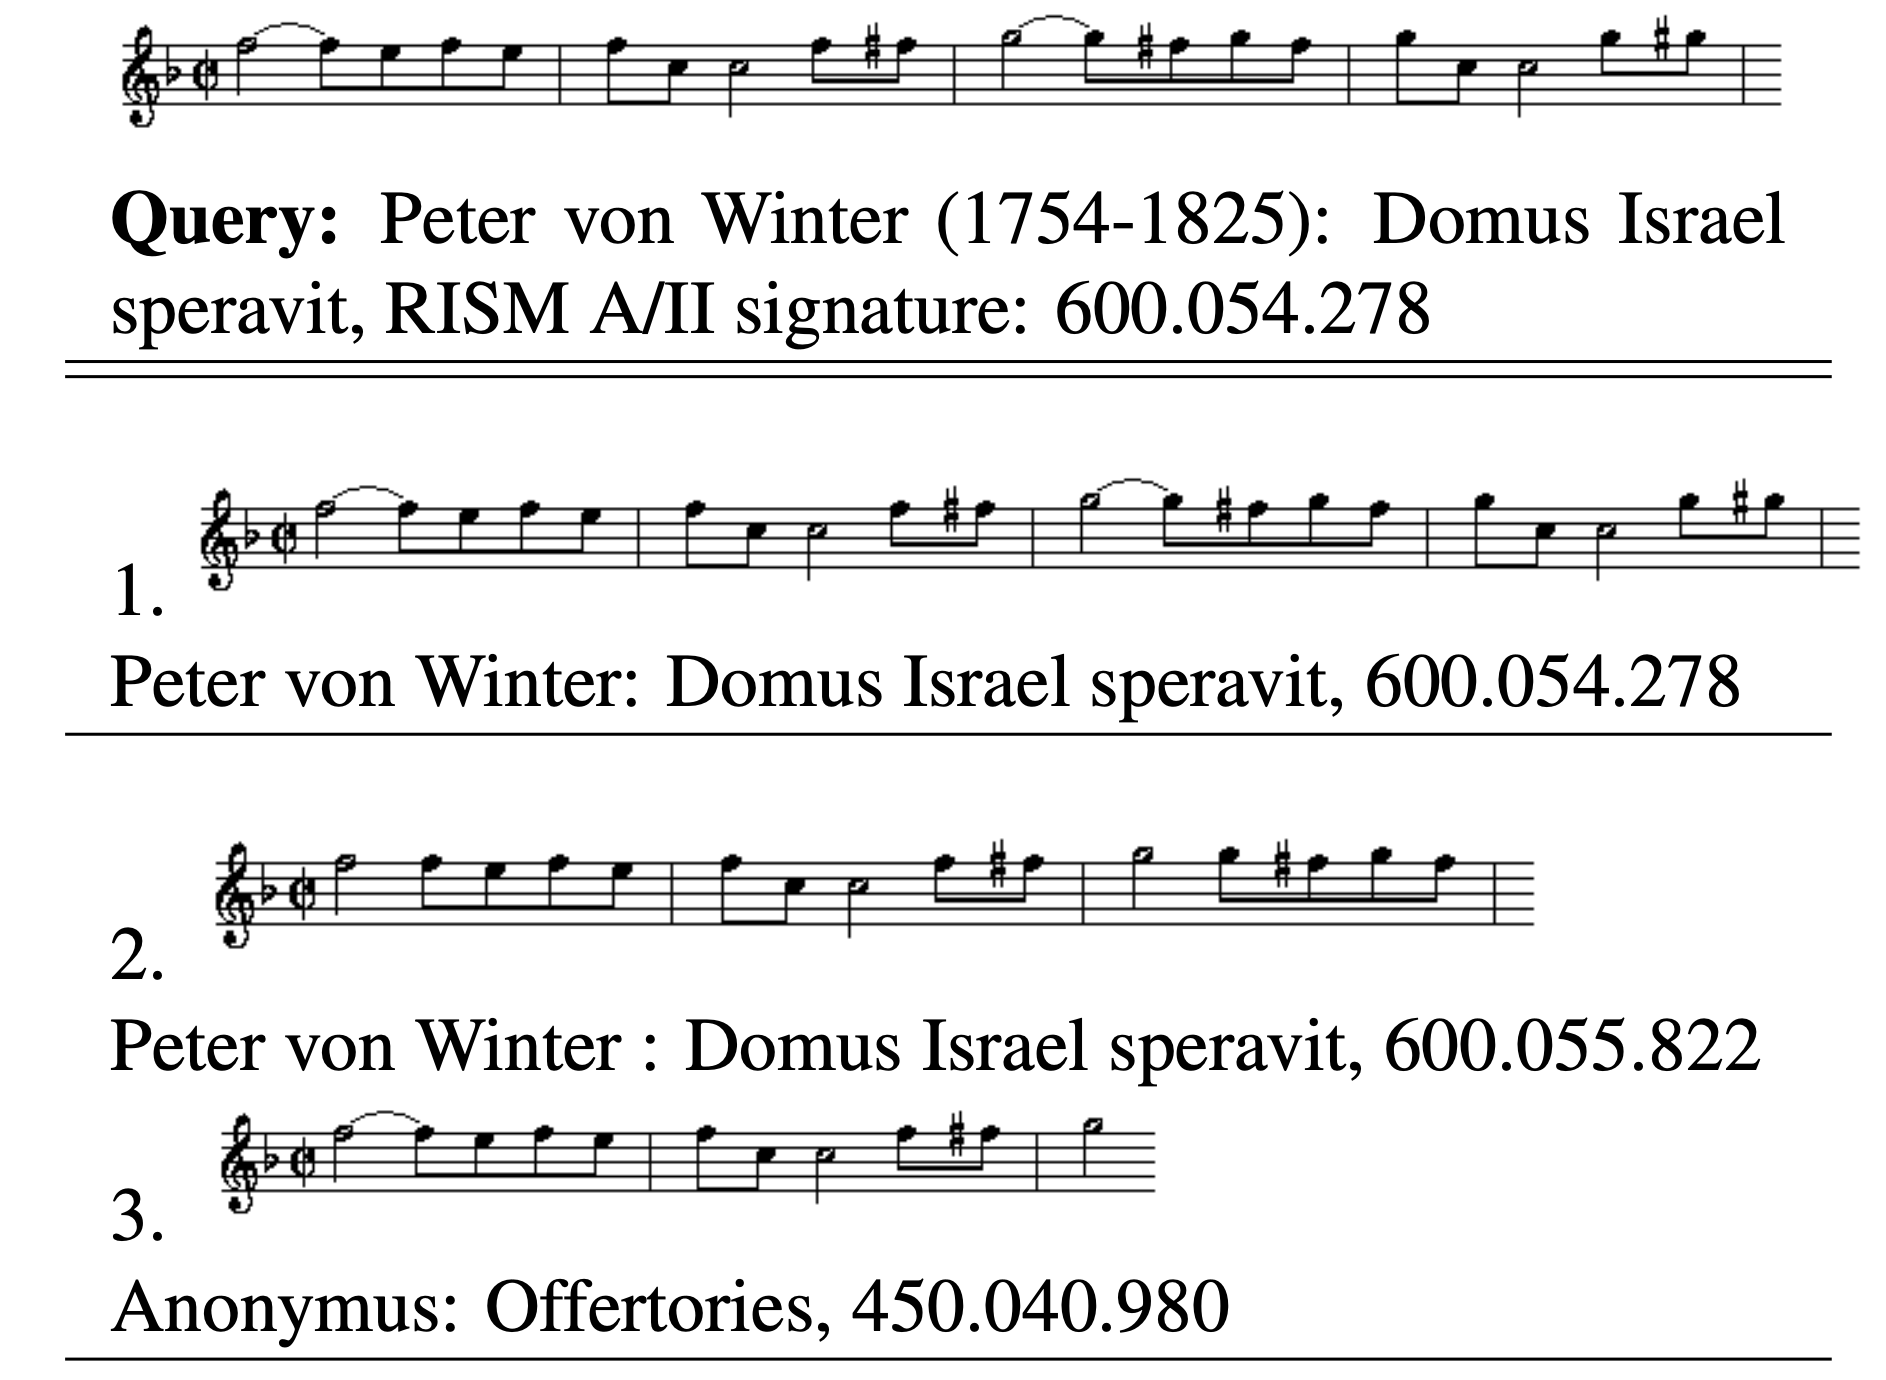
\includegraphics[width=200px,height=100px,keepaspectratio]{one_of_two_point_four_point_four}
			\caption{Ground Truth for Winter: “Domus Israel speravit \cite{two_point_four_point_four}}
		\end{figure}


 		In \cite{two_point_four_point_four} 31 experts were asked to order relevant documents to the given query in \textbf{Fig. 1}. The second and the third documents in the resulting list differ from the given query in such small ways , that it was hard to conclude a total order among results.

 		To emphasize the group boundaries better , Typke, Veltkamp, Wiering \cite{two_point_four_point_four} introduces a new measure called Average Dynamic Recall. 

		\subsection{Average Dynamic Recall}
			
			
			Authors mention nine criteria that they considered when they introduced ADR , among which we want to list the following :

			\begin{itemize}
				\item The measure doesn't need the ground truth to be completely ordered
				\item Violations of the correct order should be punished if they happen across group boundaries.
				\item Groups closer to the beginning of the list should have a higher influence on the overall scoring.
			\end{itemize}

			In comparison to standard measures such as recall and precision , ADR is specifically tailored for partially ordered lists. As to how the overall scores are given , the number of relevant documents is at the beginning is so much as there are documents within the first group. When this group of elements is completely retrieved , the number of relevant documents will get larger by adding the next group about which it is known that there is evidence that documents do differ in terms of median ranks.

			The ADR is calculated over the sum of recall values over number of iterations.     

	\section{Evaluation}
		\subsection{The graph based algorithm of Orio et al.}
			For the evaluation author used the RISM A/II collection from MIREX 2005  , which we  presented in the previous section.


			\begin{figure}[h!]
			\centering
			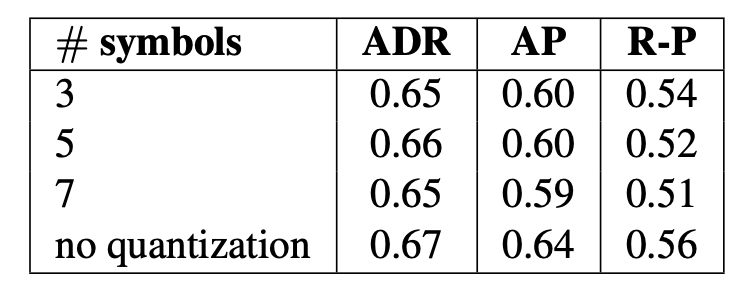
\includegraphics[width=200px,height=100px,keepaspectratio]{one_of_two_point_four}
			\caption{Manual segmentation using alphabets of different sizes \cite{two_point_four}}
			\end{figure}


			Figure 1 shows the results of quantization with alphabets of various sizes. Quantization can be seen as a function that projects a given melody onto another. As an example to a quantization with 3 symbols can be a function that projects onto the alphabet {'up','down','repeat'}. We observe that reducing a melody into simpler melody , results in loss of result quality , though not significant enough in some cases. Where memory size plays a significant role , quantization can be a preferrable process.   

			\begin{figure}[h!]
			\centering
			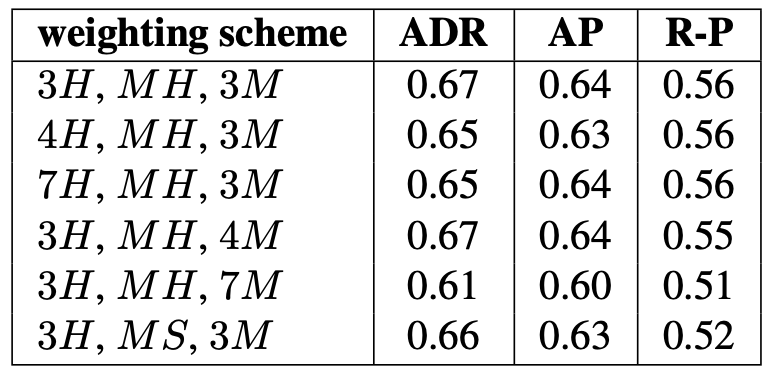
\includegraphics[width=200px,height=100px,keepaspectratio]{three_of_two_point_four}
			\caption{Different segmentation techniques with no quantization \cite{two_point_four}}
			\end{figure}

			Figure 2 shows use of different weight measures. As aforementioned weight measures are important when choosing the more important note among other notes in a measure. For harmonic weight the authors experimented with groupings of 3M,4M or 7M. While reducing the different harmonic functionalities into one larger group , it is important to make such assumptions , that result in a grouping with the least amount information loss. With the same consideration melodic weights have been grouped together in terms of their intervalic function. As to metric weight , there are two different schemes that are proposed : (1) A simple subdivision in terms of strong and weak beats and (2) \textit{"a hierarchical organization depending on the position in the measure"}. It can be observed that , even though the differences are not significant enough , the better results are obtained when weighting is based on more generalizing schemes.

			Authors observe that the size of the graph grows in a sublinear fashion , when new documents are introduced to the graph.   

\subsection{Urbano MelodyShape}
            In the initial paper of 2011, where Urbano et al. first proposed to compare melodies based on their shape, the authors tested their implementation against the RISM A/II collection from MIREX 2005 and compared their results to the results of the competing algorithms from 2005 \cite{five_point_five}. As can be seen in Fig 6, they performed best in 5 out of 11 queries and averaged the highest ADR score overall. 
        \begin{figure}[h!]
			\centering
            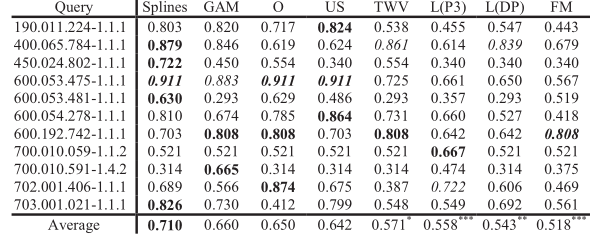
\includegraphics[width=350px,height=160px,keepaspectratio]{one_of_five_point_five}
			\caption{Spline based approach tested against the evaluation set of the MIREX 2005 competition and compared to the other contestants. \cite{five_point_five}}
        \end{figure}
            The algorithm used was later improved upon and very similar to the time system we presented earlier, using the area between two splines and a local alignment approach to determine similarity. Based upon this system Urbano developed the ShapeH and Time systems  and competed in the 2010-2015 editions of the MIREX Competition, with all submitted systems always placing in the top spots. 
        \begin{figure}[h!]
			\centering
            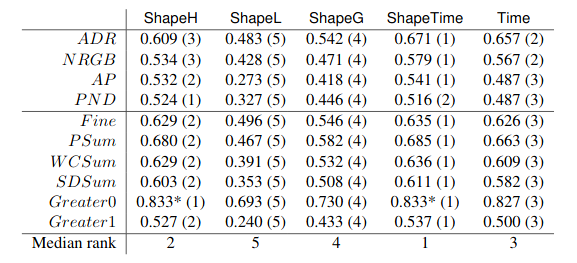
\includegraphics[width=250px,height=125px,keepaspectratio]{urbano_mirex_2012_results}
			\caption{Results for the submissions by Urbano to the 2012 MIREX Competition \cite{five_point_four}}
        \end{figure}
        \begin{figure}[h!]
			\centering
            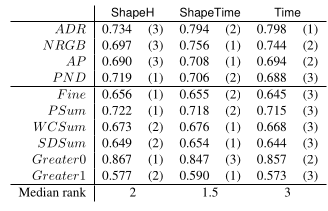
\includegraphics[width=200px,height=100px,keepaspectratio]{urbano_mirex_2013_results}
			\caption{Results for the submissions by Urbano to the 2013 MIREX Competition \cite{five_point_three}}
        \end{figure}
        \begin{figure}[h!]
			\centering
            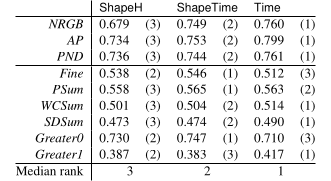
\includegraphics[width=200px,height=100px,keepaspectratio]{urbano_mirex_2014_results}
			\caption{Results for the submissions by Urbano to the 2014 MIREX Competition \cite{five_point_two}}
        \end{figure}
        
        However although the systems by Urbano seem to be performing best in the competition, the results themselves vary from year to year with the algorithms not really having changed, as Urbano himself points out in his paper to the 2014 competition \cite{five_point_five}.  Whilst the ShapeTime system, as mentioned in chapter 2.2, usually achieved the best results on average, it was outperformed by the time system in 2014 (Fig.9). Scores in single categories also varied with the ShapeH system achieving an ADR score of 0.609 in the 2012 competition (Fig.7) and achieving a a score of 0.734 in the same categorie the following year (Fig.8). These inconsistent scores along with the MIREX competition not releasing the used queries since 2010 make comparing submissions from different years rather difficult.




	\section{Discussion}

	There still seem to be  several problems in the field of symbolic melodic music similarity.
	Seeing as there is no definitive definiton for what exactly constitutes music similarity and no agreed upon data set existing, against which methods can be evaluated,  comparing different methods is challenging, if not impossible. Even results from different years of the MIREX competition can hardly be compared to each other. Furthermore there are only limited real world applications for algorithms that only compare monophonic pieces, as most music consists of polyphonic compositions. 
	- Field suffers from no Ground Truths -- big database needs to be established against which all algorithms are evaluated. 
	- Most methods are monophonic in nature -- need for shift to more polyphonic oriented algorithms.
	- MIREX Results inconclusive. 
	

	\begin{thebibliography}{7}
	
	\bibitem {kil:civ}
	A. D. Kilmer and M. Civil, 
	"Old Babylonian Musical Instructions Relating to Hymnody" 
	Journal of Cuneiform Studies 38, 
	no. 1 (Spring 1986): 94-98.

	\bibitem{five_point_two} 
	J. Urbano. MelodyShape at 
	MIREX 2014 Symbolic Melodic Similarity. 
	Technical report, Music Information Retrieval Evaluation eXchange, 2014.

	\bibitem{two}
	Symbolic Melodic Similarity: State of the Art and Future Challenges
	Valerio Velardo,Mauro Vallati and Steven Jan
	Computer Music Journal, 40:2, pp. 70–83, Summer 2016 doi:10.1162/COMJ a 00359
	2016 , Massachusetts Institute of Technology.v

	\bibitem{two_point_four} Orio, N., and A. Rodá. 2009. “A Measure of Melodic Similarity Based on a Graph Representation of the Music Structure.” In Proceedings of the International Conference for Music Information Retrieval, pp. 543– 548.

	\bibitem{three} Typke, Rainer. (2007). Music Retrieval based on Melodic Similarity.

	\bibitem{one} Greg Aloupis, Thomas Fevens, Stefan Langerman, Tomomi Matsui, Antonio Mesa, Yurai Nunez, David Rappaport, and Godfried Toussaint, "Algorithms for Computing Geometric Measures of Melodic Similarity" Computer Music Journal, Vol.30, No. 3 (Autumn, 2006), pp. 67-76

	\bibitem{two_point_four_point_four} R. Typke, R. C. Veltkamp and F. Wiering, "A Measure for Evaluating Retrieval Techniques based on Partially Ordered Ground Truth Lists," 2006 IEEE International Conference on Multimedia and Expo, Toronto, Ont., 2006, pp. 1793-1796.
	
	\bibitem{five_point_five} J.Urbano, J. Morato, J. Lloréns, S. Sanchez Cuadrado, "Using the Shape of Music to Compute the Similarity between Symbolic Musical Pieces", International Symposium on Computer Music Modeling and Retrieval, pp. 385-396, 2010
	
	\bibitem{five_point_three} J. Urbano. MIREX 2013 Symbolic Melodic Similarity:
A Geometric Model supported with Hybrid Sequence
Alignment. Technical report, Music Information Retrieval Evaluation eXchange, 2013.

 \bibitem{five_point_four} J. Urbano, J. Lloréns, J. Morato, and S. Sánchez 
Cuadrado. MIREX 2012 Symbolic Melodic Similar-
ity: Hybrid Sequence Alignment with Geometric Rep-
resentations. Technical report, Music Information Re-
trieval Evaluation eXchange, 2012.
	

	\end{thebibliography}

	
\end{document}
